\chapter{CC-Inclusive Cross Section Selection Filter} \label{ch:meas}
The CC-Inclusive cross-section selection I and selection I modified filters used in this analysis will be described in the following sections below. These filters are an expansion of the Neutrino ID filter. The work done in this thesis was to further improve these selections by increasing both efficiency and purity as well as increasing acceptance without further affecting the kinematic distributions of the selected neutrino events.
 
MicroBooNE requires fully automated event reconstruction and selection algorithms for use in the many physics measurements being worked on to date due to the large data rate MicroBooNE receives. Being able to automatically pluck out the neutrino interaction among a sea of cosmics proved to be challenging but was accomplished. MicroBooNE has developed two complementary and preliminary selection algorithms to select charged-current $\nu_{\mu}-Ar$ interactions. Both are fully automated and cut based. The results of this thesis will focus on selection I and selection I modified and will focus on further improving these algorithms using Convolutional Neural Network (CNN) implementations. These selections identify the muon from a neutrino interaction without biasing towards track multiplicity. To combat cosmic and neutral current background, the analysis is strongly biased towards forward-going long tracks which are contained. This limits phase space and reduces acceptance. 

\section{Data and MC Processing Chain}
The data used for this analysis were based on hardware and software triggers. Events used came from the \textit{BNB\_INCLUSIVE} and \textit{EXT\_BNB\_INCLUSIVE} streams and were used for signal and background. The \textit{BNB\_INCLUSIVE} stream is chosen by requiring that the hardware trigger bit is fired and that the event passed an optical software trigger within a BNB spill timing window. The \textit{EXT\_BNB\_INCLUSIVE} stream requires the EXT hardware trigger to fire as well as pass the same optical software trigger within a BNB spill size timing window similar to the \textit{BNB\_INCLUSIVE}. 

The two MC samples used in this analysis and for determining selection efficiencies and purities were GENIE BNB neutrino interactions with CORSIKA cosmic ray overlay within the readout window and inTime CORSIKA cosmic rays. The MC samples generated used \textit{\textbf{uboonecode v04\_36\_00}} and are based on the following packages:
\begin{itemize}
\item{larsoft v04\_36\_00}
\item{GEANT v04\_09\_06\_p04d}
\item{GENIE v02\_08\_06d}
\item{GENIE xsec v02\_08\_06a}
\item{pandora v02\_03\_0a}
\item{CORSIKA v07\_4003}
\end{itemize}

Both data and MC samples were processed using the same reconstruction release, \textit{\textbf{uboonecode v05\_08\_00}} and the fcl files used for reconstruction are listed below:
\begin{itemize}
\item{MC fcl files}
\begin{itemize}
\item{reco\_uboone\_mcc7\_driver\_stage1.fcl}
\item{reco\_uboone\_mcc7\_driver\_stage2.fcl}
\end{itemize}
\item{Data fcl files}
\item{reco\_uboone\_data\_Feb2016\_driver\_stage1.fcl}
\item{reco\_uboone\_data\_Feb2016\_driver\_stage2.fcl}
\end{itemize}

On top of the hardware and software triggers, the data also had to pass more criteria to be identified as part of the good run list. The criteria is detailed below.
\begin{itemize}
\item{\textbf{Detector conditions:} the detector has to be in a good operating condition. The detector conditions are read from the slow monitoring database and are required to be within the alarm thresholds. The variables of interest for events passing the good run list criteria incluse DAQ, PMT, HV, Drift HV, wire bias, electron lifetime and detector power. These conditions need to be met on a run-by-run basis in order to pass the selection.}
\item{\textbf{Data quality:} normal and stable behavior for basic reconstruction quantities. These reconstruction variables include average number of tracks, hits, and flashes in each event, the average length of tracks, the average amplitude and area of hits, the average PE and the average spread of each one of these quantities.}
\item{\textbf{Beam Conditions:} the BNB must be on and stable and the POT per spill needs to above the intensity threshold. Beam quality conditions include checking the fraction of proton beam interacting within the target, the horn current, and the intensity of protons per spill. The final sample is $5 * 10^{19}$ and a per-spill intensity of $4 * 10^{12}$}
\item{\textbf{Run processed:} the full run must be processed completely without missing subruns or crashes in the data processing.}
\end{itemize}

The selection begins with a cut that requires an optical flash greater than 50 photo electrons (PE) in the 1.6 $\mu$s beam window. Next, two or more 3D reconstructed tracks must be within 5 cm from a 3D reconstructed vertex. The most forward going track vertex-track association is then selected for further cuts. The vertex from the chosen association must be in the fiducial volume, and the longest track from this association must be matched to a flash 80 cm in z. Lastly the longest track must be contained and longer than 75 cm.       

\section{Normalization of data and MC}
The off-beam sample is used to measure beam unrelated backgrounds. For normalization, one needs the total number of BNB spills \textit{$(N_{BNB}$} and the total number of external triggers. The BNB spills used need to pass the beam quality cuts. The normalization factor is then \textit{$N_{BNB}/N_{EXT}$} which is 1.23. 

To normalize generated BNB MC events to POT, we used the following:
\begin{itemize}
\item{ $5 * 10^{19} POT = 41524.3$ generated events}
\end{itemize}
where this scaling factor only applies to mcc7 generated events. The inTime cosmic sample is normalized with respect to the open cosmic sample so an understanding of both is necessary. The POT per beam spill for mcc7 BNB samples is $5 * 10^{12}$. To calculate how many spills are necesary to produce a specific POT one would multiply the total POT by the averge 1/POT per spill. For a total POT of $5 * 10^{19}$ the amount of spills necessary is $\frac{5 * 10^{19}}{5 * 10^{12}} = 1 * 10^7$. This is only one in ~241 events therefore each cosmic event needs to be scaled up by a factor of 240.8 when comparing to BNB MC. For inTime cosmics however, two filters are applied to reduce computing and processing time and only leave cosmics that will interact within the detector. The passing rate after these two filters is 0.02125, therefore the total inTime cosmic scaling factor to compare inTime cosmics to BNB is $0.02125 * 240.8 = 5.12$.

%The efficiency and purity are used as performance values of selection I. Efficiency is described as the number of selected true $\nu_{\mu}$ CC events divided by the number of expected true $\nu_{\mu}$ CC events. The purity is described as the number of selected true $\nu_{\mu}$ CC events divided by the sum of itself and all the backgrounds. The efficiency of selection I is 12\% and the purity is 39.7\%. The poster related to this proceedings will focus on the last cut which requires the longest track to be longer than 75 cm. This cut has a passing rate of 30\% w.r.t the previous cut and is implemented in part to separate charged-current events from neutral-current events that mimic our signal. Implementing a CNN for $\mu-\pi$ separation picks out differences in these two particles that are track range independent therefore eliminating the need for the 75 cm track length cut and increase efficiency and passing rate at low muon momentum. Figure \ref{fig:track} shows the track distribution of selection I and the lack of data below  the 75 cm track length cut. Figure \ref{fig:eff} shows the efficiency of selection I as a function of muon momentum.     
\begin{figure}[htp!]
\centering
	\begin{subfigure}[b]{.4\textwidth}
	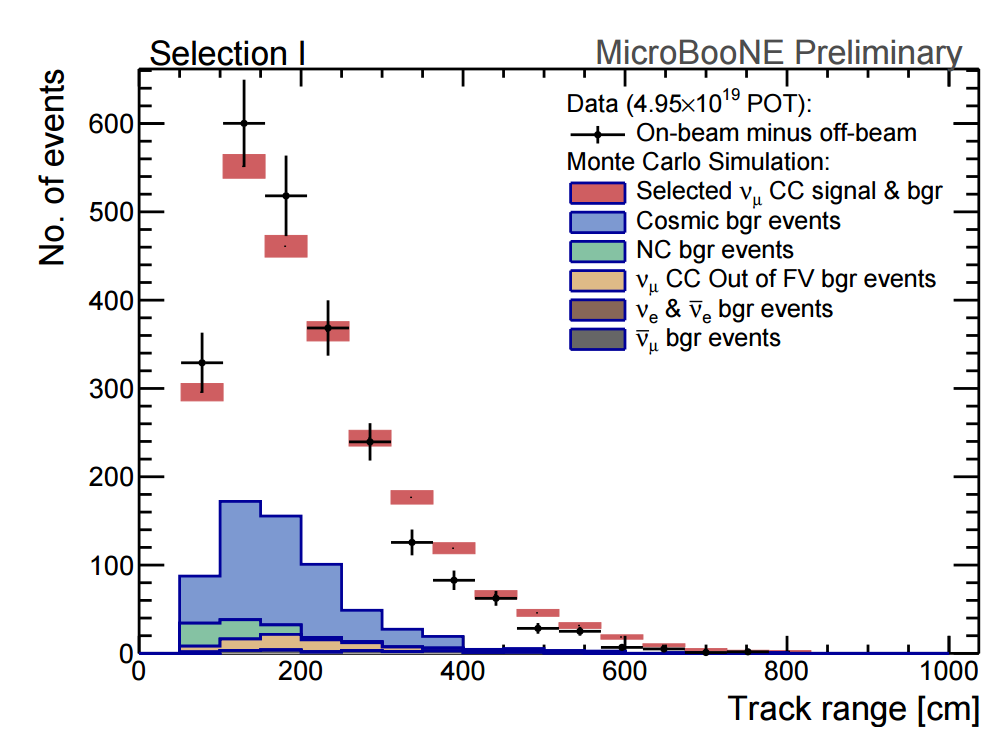
\includegraphics[width=\textwidth]{figs/track_distribution.png}
	\caption{Track range distribution of selection I}
	\label{fig:track}
	\end{subfigure}
	\quad	
	\begin{subfigure}[b]{.4\textwidth}
	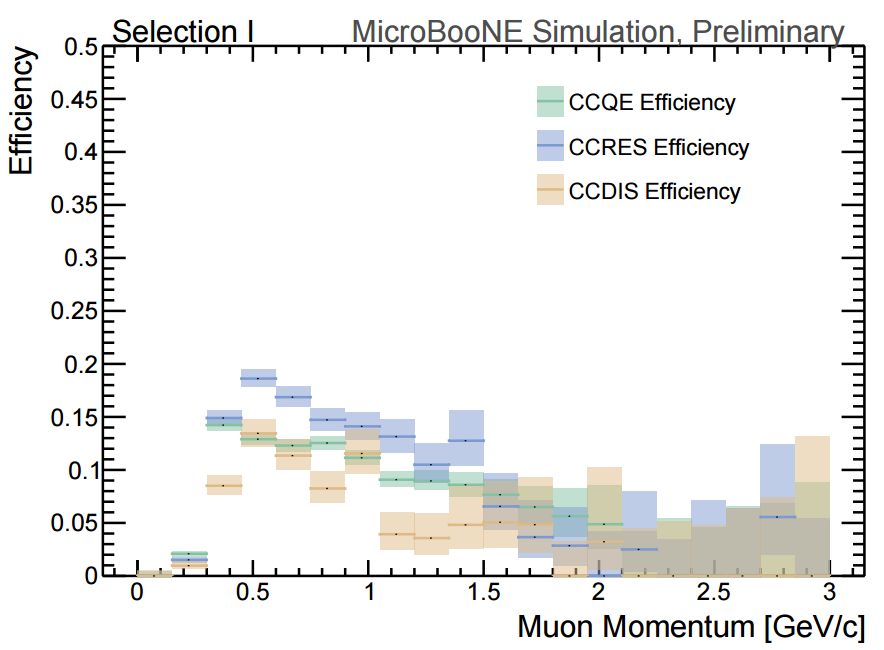
\includegraphics[width=\textwidth]{figs/efficiencyvsmom.png}
	\caption{Selection efficiency as a function of the true muon momentum}
	\label{fig:eff}
	\end{subfigure}
	\quad
\label{fig:distributions}
\caption{\ref{fig:track} Track range distribution for selection I. The track range is defined as the 3D distance between the start and end of the muon candidate track. No data is shown below 75 cm due to the track length cut described previously. \ref{fig:eff} Efficiency of the selected events by process quasi-elastic (QE), resonant (RES), and deep-inelastic (DIS). Statistical uncertainty is shown in the bands and the distributions are a function of true muon momentum. The rise of the efficiency between 0 GeV and 0.5 GeV is due to the minimum track length cut and the decreasing efficiency for higher momentum tracks is caused by the containment requirement.} 
\end{figure}
\section{Optical Software Trigger and Reconstruction}
\section{TPC Reconstruction}
\section{Event Selection}
%\section{The importance of $\mu/\pi$ separation}
